% part_B: 원문 8쪽 III절 ~ 13쪽 IV-D절 끝 (그림 5, 6 / 표 VII, VIII)

\section{직관 기반 의미 통신}

\subsection{데이터 복원을 위한 의미 통신}

직관 기반 의미 통신(SC)은 의미 부호기와 의미 복호기로 이루어진 종단 간 구조 위에 세워졌으며, 처음에는 단일 모달리티 데이터를 전송하고 복원하기 위해 개발되었다.
여러 모달리티 가운데 이미지, 텍스트, 음성이 흔히 쓰였는데, 주된 이유는 이들이 높은 데이터 전송률을 요구하기 때문이다.
특히 결합 원천-채널 부호화(JSCC, joint source-channel coding)에 기반한 종단 간 딥러닝 방식이 널리 쓰인다.

\paragraph{1) 이미지 복원}
최초의 방식인 DeepJSCC는 합성곱 신경망(CNN, convolutional neural network) 기반 오토인코더 구조로 무선 채널에서 이미지를 효율적으로 전송할 수 있음을 보였다 [5].
원천 부호화와 채널 부호화를 따로 수행하는 기존 전송 시스템과 달리, 이 방식은 두 부호화를 결합해 최적화함으로써 복원에 필요한 특징을 보존한다.
예를 들어 낮은 SNR에서 복원 이미지는 기존 분리 설계에서 나타나는 급격한 절벽 효과(cliff effect)를 보이지 않는다. 그 대신 전체 객체 구조는 유지한 채 미세한 질감을 점차 잃는다.
이를 바탕으로 이미지 복원을 위한 다양한 SC 방식이 제안되었다 [6], [7].
그 가운데 되먹임을 쓰는 딥러닝 기반 JSCC(DeepJSCC-f, deep learning-based JSCC with feedback) 방법 [45]은 채널 출력을 되먹임으로 활용해 강건성을 높였다.
DeepJSCC-f 방법은 전송 이미지와 복원 이미지 사이의 평균 제곱 오차(MSE, mean-squared error) 손실을 최소화해, JPEG2000과 저밀도 패리티 검사(LDPC, low-density parity-check) 방법보다 높은 최대 신호 대 잡음비(PSNR, peak signal-to-noise ratio)를 달성했다.
[6]에서는 변하는 채널 조건에서 복원의 강건성을 높이기 위해 어텐션 딥러닝 기반 JSCC(ADJSCC, attention deep learning-based JSCC) 방법을 도입했다.
ADJSCC 방법은 어텐션 가중치를 써서 서로 다른 신호 대 잡음비(SNR, signal-to-noise ratio) 영역 전반에서 강건성을 유지한다.
CNN으로도 이미지를 효과적으로 복원할 수 있지만, 트랜스포머(Transformer)를 쓰는 방법 [46]이 CNN보다 이미지를 더 잘 복원할 수 있음이 확인되었다.
구체적으로, 최근 연구 [46]은 합성곱 층을 Swin Transformer 층으로 바꾸어 SC 성능을 높였다.

\paragraph{2) 텍스트 복원}
SC 방법은 텍스트 데이터 처리에서 큰 개선을 보였다.
예를 들어 DeepSC [9]는 텍스트 데이터에 의미 이해를 적용해 핵심 정보를 전송하도록 개발되었다.
이 방법은 DeepJSCC 체계 안에서 의미 정보를 부호화하므로, 기존 무선 통신보다 텍스트를 더 효과적으로 압축해 전송한다.
구체적으로 DeepSC는 트랜스포머로 의미 특징을 부호화하며, 비트를 정확히 복구하는 대신 문장의 의미를 보존하도록 최적화된다.
그 결과 복호된 문장은 원래 의미를 유지하면서도 다른 단어를 쓸 수 있다.
DeepSC 방법은 자원이 제한된 사물 인터넷(IoT, Internet of Things) 기기에서도 SC가 가능하도록 더 개선되었으며, 이를 L-DeepSC라 한다 [47].
L-DeepSC 방법은 가지치기(pruning)로 중복 노드와 가중치를 없애, 자원이 제한된 IoT 기기에 적합함을 입증했다.
기존 DeepJSCC 방법에 기반한 텍스트 복원도 효과적일 수 있지만, 문장마다 담긴 의미 정보의 차이를 무시하고 고정된 자연어 처리(NLP, natural language processing) 트랜스포머 층에 의존한다는 단점이 있다.
이 문제를 해결하기 위해 범용 트랜스포머(UT, universal Transformer)에 기반한 SC 시스템이 제안되었다 [48].

\paragraph{3) 음성 복원}
음성 SC의 초기 시도는 DeepSC-S라는 JSCC 구조에서 시작되었다 [8].
DeepSC-S 모델은 압축-여기(SE, squeeze-and-excitation) 어텐션 네트워크를 써서 음성 신호에서 의미상 중요한 특징에 가중치를 준다.
음소 성분처럼 발화 내용을 이해하는 데 중요한 음성 특징은 보존하고, 침묵과 배경 잡음은 대부분 억제한다.
후속 연구 [49]에서는 스펙트럼과 텍스트 시퀀스를 정렬하는 연결주의 시간 분류(CTC, connectionist temporal classification) 모듈을 써서 DeepSC-S 모델을 개선했다.
음성 복원을 위해 음성을 텍스트로 바꾸고(S2T, speech to text) 다시 텍스트를 음성으로 바꾸는(T2S, text to speech) 방법도 제안되었다.
S2T와 T2S 과정을 쓰는 초기 SC 체계 [50]에서는 송신기에서 음성을 텍스트 정보로 바꾸고, 수신기에서 이를 다시 음성으로 복원한다.
이 과정에서 시스템은 음색이나 화자 정보처럼 인식에 불필요한 요소를 제거해 대역폭을 줄인다.
이 구조를 발전시킨 것이 DeepSC-TS [51]이다.
DeepSC-TS 방법은 창(window) 기반 어텐션 메커니즘을 써서 음성의 장기 특징과 단기 특징을 모두 포착했다.

\subsection{과업 지향 통신을 위한 의미 통신}

SC의 데이터 복원 기술이 발전하면서, 데이터를 복구하기보다 특정 하위 과업(downstream task)을 완수하는 데 초점을 둔 과업 지향 통신에 대한 관심도 함께 커졌다.
과업 지향 통신을 지원하기 위해, SC는 송신기의 데이터 획득·의미 부호화부터 수신기의 과업 수행까지를 종단 간으로 최적화할 수 있도록 확장되었다.
과업 지향 의미 통신(TOSC, task-oriented SC)에서는 과업과 관련된 정보만 보내 중복을 최소화하고, 전송을 과업 목표에 맞춰 효율을 높인다.
예를 들어 원격 이미지 분류 과업에서 송신기는 전체 이미지를 복원하는 데 필요한 특징이 아니라, 클래스 레이블을 결정하는 데 필요한 저차원 특징만 보낸다.

\paragraph{1) 엣지 추론}
TOSC에서 엣지 추론을 위해 연구된 주요 방식으로는 정보 병목(IB, information bottleneck) 기반 특징 압축, 분산 학습, 모바일 엣지 컴퓨팅(MEC, mobile edge computing) 오프로딩이 있다.
특히 이 가운데 IB 기반 방법은 중복을 최소화하면서 과업과 관련된 정보를 추출할 수 있어 주목받았다.

IB 기반 방법 [52]는 특징과 레이블 사이의 상호 정보를 최대화하는 한편, 특징과 입력 데이터 사이의 상호 정보는 최소화한다.
계산 복잡도를 줄이기 위해 [52]에서는 변분 IB(VIB, variational IB)를 채택했다.
분산 IB(DIB, distributed IB)에 기반해 여러 기기가 협력하는 엣지 추론 체계도 제안되었다 [53].
IB 기반 추론은 [54]에서 비디오 데이터로도 확장되었다.
이 연구는 시간 엔트로피 모델과 시공간 융합 모듈을 갖춘 결정적 IB(deterministic IB)로 프레임 간 특징 상관을 활용해 비디오 분석 성능을 높였다.

[55]에서는 무선 공중 계산(over-the-air computation)을 써서 여러 기기의 특징 전송을 무선 채널 위에서 선형으로 합산했다.
이 SC 기반 엣지 추론은 판별 이득(discriminant gain)을 최대화하도록 송신기 프리코딩과 수신기 빔포밍을 결합해 최적화함으로써 성능을 높인다.
시스템 관점에서는 IB를 쓰는 분산 학습·분산 실행 체계 [56]가 무선 프런트홀을 거쳐 엣지 기기와 서버 사이의 분산 학습을 효율적으로 수행하게 해 준다.
또 다른 연구는 IoT 네트워크에서 다중 사용자 스케줄링과 전력 할당에 초점을 두었다 [57].
알고리즘의 병렬성이 높아, 이 방법은 최신(SOTA, state-of-the-art) 알고리즘보다 엣지 학습 과업의 성능을 높이는 것으로 나타났다.

\paragraph{2) 다중 모달리티 과업}
SC가 발전하면서 제약 조건에서도 음성과 이미지 데이터를 높은 처리량으로 전송할 수 있게 되었다.
이에 따라 다중 모달 전송을 위한 다양한 TOSC 연구가 제안되었다.

Xie 등 [58]은 다중 과업을 위한 TOSC 체계를 제시했다.
이 TOSC 체계에서는 층별 트랜스포머와 메모리·어텐션·합성(memory, attention, and composition) 네트워크로 데이터를 융합하고 다중 모달 특징을 추출한다.
DeepSC-ST [24]는 음성 입력을 바탕으로 텍스트와 음성 출력을 지원하는 다중 모달 TOSC 체계로 제안되었다.
텍스트 특징과 메타데이터만 전송하므로, 음성 복원 성능을 유지하면서도 대역폭을 크게 줄일 수 있다.
DeepSC-ST 같은 과업 특화 모델은 새 과업마다 재학습이 필요해 학습 복잡도 부담이 커진다.
이 복잡도 문제를 극복하기 위해, 딥러닝 기반 SC 시스템을 통합한 U-DeepSC [25]가 제안되었다.
그러나 학습 중에 하위 과업을 특정할 수 없으면 과업 특화 최적화가 어려워진다.
이 경우 송신기는 과업과 독립적인 의미 표현을 보내고, 수신기가 이를 하위 과업에 어떻게 쓸지 결정한다(IV절과 V절 참조).
성능은 과업별 정확도가 아니라 의미 유사도나 의도 정렬(intent alignment) 같은 과업 무관(task-agnostic) 지표로 평가한다(VI절 참조).

다중 모달 데이터에 대한 연구는 자원이 제한된 환경에도 적용되었다.
네트워크의 대역폭 효율을 높이기 위해, 대규모 다중 모달 모델로 과업 지향 정보만 전송하는 TOSC 체계 [59]가 제안되었다.
마찬가지로, 다중 모달 데이터를 의미 수준에서 처리해 임무를 효율적으로 수행하는 TOSC 시스템 [60]도 제안되었다.

\paragraph{3) 과업을 위한 적응형 압축}
제약이 있는 통신 시스템에서 TOSC를 구현하면, 기기의 자원이 한정되어 있어 전송 오버헤드가 부담이 될 수 있다.
특히 SC에서는 고정된 특징 길이나 정적 특징 압축이 일반적인데, 이는 유연한 의미 전송을 가로막을 수 있다.
이를 해결하기 위해 TOSC에서 적응형 SC에 대한 다양한 연구가 활발히 진행되었다.

초기 적응형 SC 방법은 정적 특징 압축 [52]이나 임계값 기반 적응형 특징 선택 [61]을 제안했다.
구체적으로 [52]에서는 VIB 기반 가변 길이 특징 부호화(VL-VFE, variable-length feature encoding) 체계를 제안했고, [61]은 의미 중요도에 기반한 동적 특징 선택을 제안했다.
그러나 이러한 방식은 조정(tuning)에 민감하고 사전 지식이 필요하다.
이러한 한계를 해결하기 위해 최근 연구들은 유연한 설계를 제시했다. 압축률 예측 [62], 심층 강화학습(DRL, deep reinforcement learning) 에이전트를 이용한 다중 부호책 기반 동적 부호책 선택 [63], 부분 채널 상태 정보(CSI) 조건에서의 DRL 기반 적응형 압축 제어 [64], [65]가 그 예다.
그럼에도 이러한 최근 방법은 보조 모듈 때문에 추가 메모리 오버헤드와 계산 복잡도를 일으킬 수 있다.
특히 DRL 기반 적응형 방법은 전송 슬롯마다 보조 네트워크를 실행하므로 모델 가중치와 지연이 추가된다 [63], [64].
또한 다중 전송률 방법은 전송률마다 별도의 의미 모델을 유지해야 하므로, 메모리 요구량이 지원하는 전송률 수에 비례해 선형으로 늘어날 수 있다 [63].
이러한 메모리 오버헤드는 자원이 제한된 IoT 기기에 배포하는 데 걸림돌이 될 수 있다.

\subsection{디지털 호환성을 위한 의미 통신 기법}

기존 아날로그 SC 시스템은 연속값 채널 심볼을 가정한다. 그러나 실제 통신 시스템은 이산 성상 심볼을 전송한다.
이 때문에 전송 전에 양자화가 필요하다.
양자화 연산은 파이프라인을 미분 불가능하게 만들어 단순한 경사 기반 종단 간 학습을 막고, 양자화 오차도 일으킨다.
이 문제를 해결하기 위해 기존 변조 방식과 통합할 수 있는 디지털 호환 SC 체계가 개발되었다.
예를 들어 미분 불가능한 변조 연산을 다루기 위해 다중 차수 디지털 결합 부호화-변조(MDJCM, multi-order digital joint coding-modulation) 방식 [66]이 제안되었다.
MDJCM은 여러 변조 차수를 하나로 통합하지만, 낮은 차수 변조에서는 근사 오차 때문에 성능이 손실된다.

이 한계를 더 해결하기 위해 의미 디지털 변조 성상 매핑(sDMCM, semantic digital modulation constellation mapping) 방식 [67]이 제안되었다.
벡터 양자화 변분 오토인코더(VQ-VAE, vector quantized variational autoencoder) 방법 [68]도 디지털 호환 SC에 적용할 수 있지만, 변조 차수가 바뀔 때 통계적 불일치가 생긴다.
범용 JSCC(uJSCC, universal JSCC)에 기반해 서로 다른 차수와 호환되는 방식도 제안되었다 [69], [70].
전환형 정규화(switchable normalization) 층을 넣어 통계적 불일치를 해소하고, 서로 다른 변조 차수에서도 호환 전송이 가능하게 했다.
이러한 방식은 변조 무관(modulation-agnostic) 처리나 유연한 변조 처리를 염두에 두고 설계되었지만, 페이딩 채널로 일반화하는 문제는 여전히 미해결 과제로 남아 있다.
기존 디지털 변조와 달리, 이러한 방식은 심볼 오류를 최소화하는 대신 의미 정보를 보존하도록 디지털 성상을 의미 부호기·복호기와 함께 최적화한다.

\subsection{기존 연구에서 얻은 교훈}

JSCC 체계에 기반한 직관 기반 SC 시스템은 주로 단일 과업·단일 모달리티 구성에 초점을 두어 왔다.
이 설계는 의미 목표, 모달리티, 채널 통계가 학습된 표현과 안정적으로 맞아떨어질 때 효과적일 수 있다.
그러나 운용 조건이 학습된 영역에서 벗어날수록 이러한 이점은 약해진다.
높은 SNR 환경에서는 물리적 잡음의 영향이 줄어 디지털 전송의 이점이 감소하며, 분포나 과업이 바뀌면 학습된 매핑이 의미 충실도(semantic fidelity)를 잃는 경우가 많다.

최근 SC 연구에는 트랜스포머, DRL 기반 적응, 적응형 특징 압축 같은 기법이 도입되었다.
그러나 이러한 방법은 채널 조건, 변조 방식, 모달리티, 과업이 바뀌면 재학습이 필요할 수 있다.
따라서 기존 연구는 직관 기반 SC 시스템이 정적 환경에서는 효과적이지만, 재학습이나 외부 지식이 필요한 동적 환경에서는 덜 효과적임을 시사한다.
직관 기반 SC에 관한 문헌은 표~VII에 정리했다.

\setcounter{table}{6}
\begin{table}[htbp]
\centering
\caption{직관 기반 SC 문헌 검토}
\label{tab:7}
\footnotesize
\renewcommand{\arraystretch}{1.15}
\begin{tabularx}{\linewidth}{|>{\centering\arraybackslash}p{0.2\linewidth}|>{\centering\arraybackslash}p{0.12\linewidth}|>{\centering\arraybackslash}X|}
\hline
\textbf{방식} & \textbf{참고문헌} & \textbf{특징} \\
\hline
\multirow{2}{=}{\centering 데이터 복원\\(이미지)} & [5]--[7], [45] & 종단 간 학습한 CNN 오토인코더 JSCC로 무선 채널에서 이미지를 효율적으로 전송 \\
\cline{2-3}
 & [46] & Swin Transformer 층으로 SC 성능 향상 \\
\hline
\multirow{3}{=}{\centering 데이터 복원\\(텍스트)} & [9] & 텍스트 데이터에 의미 이해를 적용해 핵심 정보 전송 \\
\cline{2-3}
 & [47] & L-DeepSC에서 가지치기 기법으로 자원이 제한된 IoT 기기에서 SC 구현 \\
\cline{2-3}
 & [48] & UT 기반 SC에서 의미 정보의 차이와 적응형 반복(recurrence) 메커니즘을 반영해 다양한 채널 조건에서 성능 향상 \\
\hline
\multirow{2}{=}{\centering 데이터 복원\\(음성)} & [8], [49] & JSCC 구조를 이용한 음성-음성 직접 복원 \\
\cline{2-3}
 & [50], [51] & 효율적 전송을 위한 음성-텍스트·텍스트-음성 기반 복원 \\
\hline
\multirow{3}{=}{\centering 엣지 추론} & [52]--[54] & 엣지 추론에서 과업과 관련된 특징을 효율적으로 표현하는 IB 기반 방식 \\
\cline{2-3}
 & [55], [56] & 물리 계층 통합과 분산 시스템 설계로 추론 효율 향상 \\
\cline{2-3}
 & [57] & 자원 할당과 확장성에 초점을 둔 대규모 IoT 네트워크용 방식 \\
\hline
\multirow{3}{=}{\centering 다중 모달리티} & [24], [58] & 특정 다중 모달 과업(예: VQA, 음성-텍스트/음성)에 맞춘 모델 \\
\cline{2-3}
 & [25] & U-DeepSC로 학습 복잡도 문제 해결, 6가지 주요 과업 동시 지원 \\
\cline{2-3}
 & [59], [60] & 대역폭과 자원이 제한된 환경을 위해 설계 \\
\hline
\multirow{3}{=}{\centering 적응형 압축} & [52], [61] & 정적 임계값이나 의미 중요도로 특징 선택 \\
\cline{2-3}
 & [62] & 선택된 압축률로 하이퍼파라미터 조정에 대한 민감도와 사전 지식 의존을 완화 \\
\cline{2-3}
 & [63]--[65] & 심층 강화학습(DRL)으로 부호책이나 압축률을 동적으로 선택 \\
\hline
\multirow{4}{=}{\centering 디지털 호환성} & [66] & 대체 학습(substitution learning) 전략으로 다양한 변조 차수 지원 \\
\cline{2-3}
 & [67] & 낮은 차수 변조 환경의 성능 저하 해결 \\
\cline{2-3}
 & [68] & 공유 신경망으로 디지털 의미 압축 적용 \\
\cline{2-3}
 & [69], [70] & 디지털 호환 SC를 위해 변조 무관 JSCC 사용 \\
\hline
\end{tabularx}
\end{table}

이러한 관찰은 직관 기반 SC 시스템의 한계를 드러낸다.
무엇보다 직관 기반 SC는 모델 매개변수에 크게 의존하므로, 의미 목표가 바뀌면 추론 성능이 떨어진다.
또한 효율적인 의미 전송만으로는 동적 환경에서 맥락을 고려한 동작을 구현하기 어렵다.
고정된 설정을 넘어 일반화하려면 SC에 추론과 지식 정렬 메커니즘이 들어가야 하며, 이것이 추론 기반 SC로 넘어가는 동기가 된다.

\section{추론 기반 의미 통신}

\subsection{맥락적 추론을 갖춘 의미 통신}

추론 기반 SC는 기존의 데이터 기반 통신에서 지식 기반 통신으로의 근본적인 전환을 뜻한다.
맥락적 추론은 추론 기반 SC의 핵심 능력으로, 송신기와 수신기가 서로의 맥락을 이해할 수 있게 해 준다.
SC에서 맥락적 추론 능력을 갖추는 방식으로는 크게 두 가지, 곧 지식 베이스(KB) 기반 추론과 인지적 추론을 생각할 수 있다.
전자는 구조화된 지식을 압축과 오류 정정에 어떻게 활용하는지에 관한 것이고, 후자는 에이전트가 서로의 상태를 어떻게 추론하는지에 관한 것이다.
이 소절에서 생성 모델은 공유 KB로서의 역할로만 등장한다는 점에 유의한다. 생성 모델을 의미 코덱으로 쓰는 연구는 IV-B절에서 따로 검토한다.

\paragraph{1) KB 기반 구조적 추론}
맥락적 추론과 압축을 위해 KB를 SC에 통합한 연구를 검토한다.
KB는 데이터 분포를 추론하는 데 그치지 않고 사실, 규칙, 온톨로지를 부호화하는 데 쓰인다.
의미 범주 예측을 돕기 위해 도입된 지식 네트워크 개념 [71]이 SC 체계에 적용되었다.
기존 SC 연구에서 KB는 시스템 요구 사항에 따라 다양한 표현 형태로 구현되었다.
지식 그래프(KG, knowledge graph) [44], [72]--[76]는 관계 추론에 널리 쓰이는 형태이지만, SC의 KB는 다른 형태도 포함할 수 있다.
구체적으로 대규모 언어 모델(LLM) 기반 KB [77], 생성 모델 [78], [79], 텍스트 말뭉치 [80]를 쓰는 SC 방법이 제안되었다.

초기 KG 기반 SC 방식은 KG 연결성 추론으로 수신기에서 왜곡된 트리플을 복구하도록 제안되었다 [72].
이어서 구조화된 지식에서 개체(entity) 추론을 수행하는 텍스트-KG(Text2KG) 및 KG-텍스트(KG2Text) 체계 [73]와, 조각난 단어들로부터 완전한 문장을 복원하는 맥락 인식 KB 방법 [74]이 개발되었다.
이러한 방식은 개체가 주어진 KG의 지식 범위를 벗어나면 메시지를 부정확하게 복원한다는 단점이 있다.
이를 완화하기 위해 KG 개체와 원천 데이터 토큰을 결합 임베딩해 누락되거나 손상된 토큰의 예측을 개선하는 방법이 제안되었다 [75].
더 최근에는 LLM을 통합해 기존 KG 기반 추론에 내재한 제약을 보완하는 KG-LLM 체계가 도입되었다 [44].
비슷한 맥락에서 LLM과 그래프 신경망(GNN, graph neural network)을 통합하는 구조 설계도 제안되었다 [76].

[77]에서는 LLM을 공유 KB로 쓰는 구조가 제안되었다.
이 구조에서 지식은 명시적 그래프가 아니라 사전 학습된 모델 매개변수 안에 암묵적으로 담기며, 프롬프트를 통해 접근한다 [77].
생성 모델을 KB로 삼으면 [78], [79], 송신기는 과업과 관련된 최소한의 단서만 전달하고 수신기는 공유 사전 분포를 바탕으로 의미상 일관된 내용을 복원한다. 따라서 메시지의 핵심 의미를 해치지 않으면서 전송 오버헤드를 줄일 수 있다.
또한 이 방식은 통신 채널 잡음에 따른 이미지 왜곡과 분류 정확도 저하 문제를 완화하며 [78], 학습 없이 실시간으로 채널에 적응할 수 있다는 장점도 있다 [79].
아울러 텍스트 말뭉치에 기반한 KB 체계는 사람이 읽을 수 있는 문장을 기본 단위로 삼고, 공유 데이터베이스에 없는 잔여 의미 정보만 전송해 통신 효율을 높인다.

\paragraph{2) 인지적 추론}
SC에서 인지적 추론이란 상대 사용자의 지식 상태를 추론하고 그에 맞춰 메시지를 조정하는 과정을 말한다.
첫 번째 연구 흐름은 맥락적 추론에 초점을 두었다. 여기서는 송신자와 수신자가 의미 표현을 반복해서 갱신하며 공유 맥락으로 수렴한다.
두 번째 흐름은 암묵적 의미의 전송에 초점을 두었다. 암묵적 의미는 수신자가 재구성해야 하는 잠재 추론 구조와 함께 부호화되어 전송된다.
마지막 흐름은 과업 효용을 높이기 위한 화용 통신(PragCom, pragmatic communication)에 초점을 두었다.

Seo 등 [13]은 상대의 상태를 미리 추론하는 과정을 SC에 적용하는 이론을 제안했다.
이 이론에서 송신자는 의미 표현을 수신자의 상태에 맞추고, 수신자는 송신자의 맥락을 추론한다.
반복적인 추론을 거쳐 양측은 필요한 비트 수를 최소화하고 신뢰성을 유지하면서 공통 맥락으로 수렴한다.
후속 연구 [81]에서는 초기 지식과 맥락이 서로 다른 상황을 위해, 베이즈 역추론에 기반한 역 맥락 추론(iCR, inverse contextual reasoning)과 역 선형 맥락 추론(iLCR, inverse linear contextual reasoning) 방법을 제안했다.
iLCR은 계산 복잡도를 줄이면서 상대 맥락 추정의 정확도를 높였다.

또 다른 연구 흐름은 수신기 쪽 추론을 활용하기 위해 암묵적 의미 구조를 전송하는 데 초점을 두었다.
암묵적 SC(iSC, implicit SC) 체계 [82]는 인과 관계를 의미 그래프로 부호화하고, 수신기는 이를 재구성해 암묵적 의미를 복구한다.
이를 바탕으로 암묵적 의미 인식 통신 체계 [83]는 그래프 기반 표현을 물리 계층 변조와 결합해 의미 그래프를 저차원 성상에 사영한다.
iSC의 아이디어를 개인화된 의미로 확장한 다층 의미 방식 [84]도 제안되었다. 이 방식은 모방 기반 추론으로 전송 의미를 사용자별 추론 선호에 맞춘다.
iSC 관련 기존 방법들은 전송 메시지에 추론 구조를 담으면 맥락에 더 잘 적응하는 SC가 가능함을 보여 준다.

PragCom은 전달되는 의미보다 과업 효용에 초점을 둔 체계로서 SC에 제안되었다 [85].
이종 통신에서는 송신자와 수신자가 공유하는 지식 표현이 없을 때 의미 불일치가 생긴다 [85].
이러한 오류를 해결하려면 의미 채널과 효과성 채널(effectiveness channel)에 대한 조정 메커니즘과 수학적 모델링이 필요하다.
\emph{마음 이론}(ToM, theory of mind) [86] 개념은 이러한 문제의 실현 가능한 해법이 될 수 있다.
PragCom에서 ToM은 송신자가 수신자의 상태를 모델링하게 해 주어 에이전트 간 의미 불일치를 줄인다.
다른 방식에서는 마르코프 결정 과정(MDP, Markov decision process) 모델링과 최적 수송(optimal transport) 방법을 채택해 의미 불일치를 완화한다 [87].
이러한 기존 연구는 PragCom이 의미 조정과 모델링을 통해 의미 불일치를 완화할 잠재력이 있음을 보여 주었다.

\subsection{생성형 AI를 갖춘 의미 통신}

제한된 통신 자원에서 의미 압축, 복원, 강건성을 높이기 위해 생성형 AI(GAI)를 SC에 통합하는 연구가 많이 수행되었다.
SC의 대표적인 방법으로는 변분 오토인코더(VAE) [88], [89], 생성적 적대 신경망(GAN, generative adversarial network) [90]--[93], 확산 모델 [94]--[97]이 연구되었다.

\setcounter{figure}{4}
\begin{figure}[htbp]
\centering
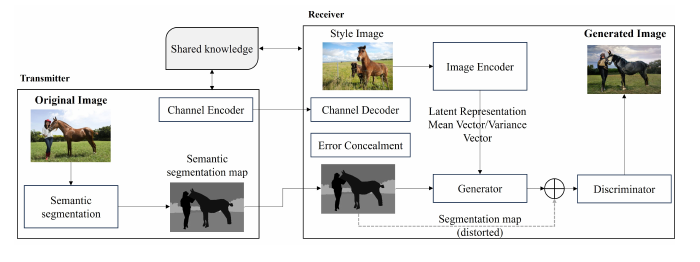
\includegraphics[width=\linewidth]{fig/fig5.png}
\caption{GAI를 갖춘 추론 기반 SC의 구조 [93].}
\label{fig:5}
\end{figure}

VAE에서는 입력 데이터를 한 번의 추론으로 압축하고 복원하므로, 지연이 짧아야 하고 대역폭이 제한된 SC에 적합하다.
잡음에 강한 마스크드(masked) VQ-VAE 체계 [88]는 송신기와 수신기가 이산 부호책을 공유해 의미 잡음을 억제하고 대역폭 사용을 줄인다.
VQ-VAE-2 [98]를 채택한 배포 후 미세 조정 가능 SC(FTSC, post-deployment fine-tunable SC) 체계 [89]도 제안되었다.
FTSC 체계에서는 복호기에서 미세 조정을 거쳐 미지의 데이터 분포에 적응함으로써 일반화 성능을 높일 수 있다.
그러나 VAE에 내재한 저차원 병목은 출력 해상도를 제한한다. 이 단점은 채널 잡음이 클 때 더 심해져 세밀한 의미 정보가 손실된다.

GAN 모델은 전송 강건성 [90], [91]과 의미 충실도 [92], [93]를 높이는 데 쓰였다.
예를 들어 텍스트 입력을 위한 GAN 기반 SC 체계가 제안되었다 [90].
이 체계는 의미 전송을 위한 부호기-복호기와, CSI 없이 왜곡을 완화하는 GAN 기반 모듈을 통합한다 [90].
또 다른 연구는 중요 영역을 보존하기 위해, 관심 영역(ROI, regions of interest)과 비관심 영역(RONI, regions of non-interest)에 기반한 내용 인식 양자화를 GAN과 통합해 적용했다 [91].
이 체계에서는 다중 스케일 GAN 판별기와 무작위 SNR 샘플링으로 열악한 채널에서도 강건성을 얻을 수 있다.
내용 인식 특징만 전송하고 수신기가 GAN으로 고해상도 이미지를 복원하는 SC 방법 [92]도 제시되었다.
마찬가지로, 그림~5에 보인 것처럼 의미 분할된 이미지만 전송해 수신기에서 이미지를 복원하는, SC 방법을 결합한 GAN 모델이 제안되었다 [93].
부분 입력에서 원본 데이터를 추론하는 이 두 방식은 부분적인 의미 입력으로부터 시각적으로 그럴듯한 내용을 재생성하므로 전송 오버헤드를 크게 줄일 수 있다.
그러나 지각적 타당성이 과업 충실도를 보장하지는 못하며, 분포 변화에 취약하다는 점 때문에 동적 무선 환경에 실제로 배포하기 어렵다.

확산 모델은 채널 손상에 대한 강건성을 높이기 위해 SC에 적용되었다.
예를 들어 채널 잡음을 완화하기 위해 채널 잡음 제거 확산 모델 [94]이 도입되었다.
마찬가지로 이미지 전송에 확산 확률 모델(DPM, diffusion probabilistic model)을 적용한 확산 SC(DiffSC, diffusion SC) 체계 [95]도 도입되었다.
이러한 장점에도 불구하고, 확산 모델은 반복적으로 동작하므로 지연 문제가 생긴다.
이 문제를 해결하기 위해 허용할 만한 품질을 유지하면서 샘플링 단계 수를 줄이는 SC 방법 [96]이 제안되었다.
비슷한 맥락에서 Grassucci 등 [97]은 자원이 제한된 환경을 위한 경량 확산 모델을 제안해, 수신기의 계산 오버헤드와 에너지 소비를 모두 줄였다.

SC에서 이 세 가지 생성 모델은 저마다 뚜렷한 강점과 한계가 있다.
VAE, GAN, 확산 기반 방법은 각각 저지연 채널, 대역폭이 제한된 채널, 심하게 손상된 채널에 맞게 구현할 수 있다.
그러나 각 방식에는 VAE의 부호책 동기화, GAN의 지각-의미 불일치, 확산 모델의 샘플링 지연처럼 실용상의 한계가 있다.

\subsection{이질성을 다루는 의미 통신}

앞의 절들은 SC 시스템의 추론 메커니즘에 초점을 두었다.
이 절에서는 추론 능력을 이종 네트워크 시나리오에 적용하는 방안을 살펴본다.

\paragraph{1) NOMA}
기존 연구의 상당수가 단일 사용자 SC에 집중했지만, 몇몇 연구는 이를 다중 사용자 환경으로 확장하는 방안을 탐구했다.
비직교 다중 접속(NOMA, non-orthogonal multiple access)은 전력 다중화로 같은 시간-주파수 자원 안에서 동시 접속을 가능하게 하므로, 다중 사용자 환경의 SC에 적합하다고 여겨진다.
[99]에서는 학습된 이산 표현과 다중 사용자 검출용 신경망을 써서 이종 사용자 데이터 형식을 지원하는 NOMA 기반 SC(NOMASC)를 제안했다.
또한 원거리장(far-field) 사용자는 SC를 쓰고 근거리장(near-field) 사용자는 기존 비트 기반 통신을 쓰는 NOMA 기반 체계도 도입되었다 [100].
전송 유연성을 더 높이기 위해 NOMA를 변형한 semi-NOMA 방법도 제안되었다 [101].

\paragraph{2) 토큰 통신}
이질성은 사용자 수준을 넘어 전송 데이터의 표현 형태에도 존재한다.
다중 접속 환경의 GSC를 위한 새로운 토큰 통신(TokCom, token communication) 체계가 제안되었다 [102].
이 체계에서 토큰은 미래 무선 네트워크에서 전송되는 의미 내용의 단위 역할을 한다.
TokCom에서는 송신기가 다중 모달 신호의 의미 내용을 부호화하고, 수신기가 맥락 정보를 이용해 이를 복구한다.
그림~6에서 보듯이, 단방향 예측은 과거 토큰을 활용해 저지연 부호화와 변조를 가능하게 한다.
반면 양방향 마스크드 예측은 전체 맥락을 써서 패킷 복구 측면의 정확도를 높인다.
[103]에 따르면 TokCom 패킷이 손상되면 메시지가 불완전해질 수 있다.
의미 오류 정정은 사전 학습된 LLM이 수행하며, 이 LLM은 주변 맥락으로부터 마스크된 단어를 예측한다.
따라서 TokCom 기반 맥락 추론은 재전송 횟수를 줄인다.

\setcounter{figure}{5}
\begin{figure}[htbp]
\centering
\begin{minipage}{0.6\linewidth}
\centering
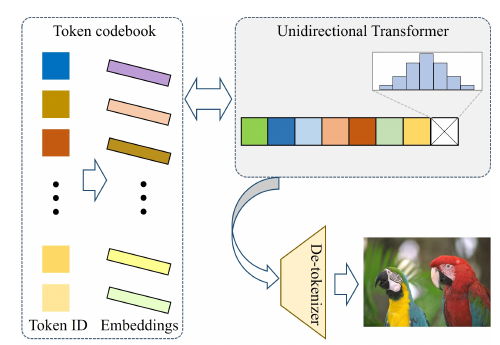
\includegraphics[width=\linewidth]{fig/fig6a.png}\\[2pt]
{\small (a) 단방향 TokCom(다음 토큰 예측)}
\end{minipage}\\[10pt]
\begin{minipage}{0.6\linewidth}
\centering
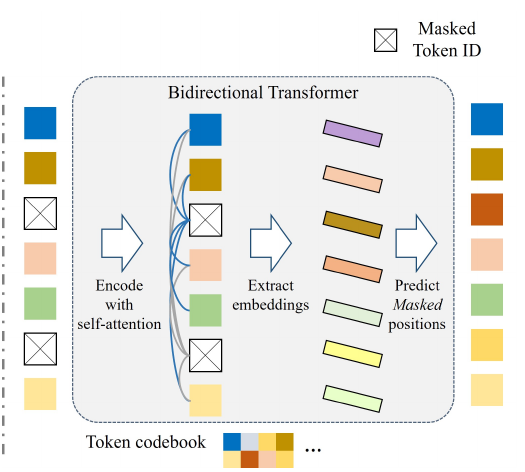
\includegraphics[width=\linewidth]{fig/fig6b.png}\\[2pt]
{\small (b) 양방향 TokCom(마스크드 토큰 예측)}
\end{minipage}
\caption{단방향 TokCom 체계와 양방향 TokCom 체계의 비교 [102].}
\label{fig:6}
\end{figure}

이러한 토큰 기반 통신 패러다임은 학계뿐 아니라 3세대 파트너십 프로젝트(3GPP, 3rd Generation Partnership Project) 같은 표준화 기구에서도 논의되고 있다 [104].
구체적으로 3GPP 시스템 구조(SA, system architecture) 그룹은 패킷이 아니라 \emph{토큰}을 기본 단위로 하여 GAI 서비스를 지원하는 다중 모달리티 트래픽 모델을 정의한다.
또한 이 연구는 토큰 크기, 토큰 중요도 같은 새로운 서비스 품질(QoS, quality of service) 지표를 도입한다.
나아가 Release~19에서는 추론 시간을 핵심 변수로 고려한다 [105].
이러한 흐름은 미래 6G 시스템이 비트 중심의 신뢰성에서 토큰 중심의 의미 신뢰성으로 옮겨 가고 있음을 보여 준다.

\setcounter{table}{7}
\begin{table}[htbp]
\centering
\caption{추론 기반 SC 문헌 검토}
\label{tab:8}
\footnotesize
\renewcommand{\arraystretch}{1.15}
\begin{tabularx}{\linewidth}{|>{\centering\arraybackslash}p{0.2\linewidth}|>{\centering\arraybackslash}p{0.12\linewidth}|>{\centering\arraybackslash}X|}
\hline
\textbf{방식} & \textbf{참고문헌} & \textbf{특징} \\
\hline
\multirow{6}{=}{\centering 맥락적 추론\\(KB 기반)} & [72]--[74] & KG로 개체 관계를 추론해 오류를 정정하고 오버헤드를 줄임 \\
\cline{2-3}
 & [75] & 토큰과 정렬된 KG 개체의 결합 임베딩으로 지식 범위 밖 사례에 대응 \\
\cline{2-3}
 & [44], [76] & KG의 사실 참조와 LLM의 맥락 해석을 결합하는 KG-LLM \\
\cline{2-3}
 & [77] & 사전 학습된 LLM을 암묵적 공유 KB로 사용 \\
\cline{2-3}
 & [78], [79] & 생성 사전 분포를 공유 KB로 써서 과업과 관련된 최소한의 단서만 전송 \\
\cline{2-3}
 & [80] & 텍스트 말뭉치를 읽을 수 있는 KB로 쓰고, 데이터베이스에 없는 과업 관련 정보를 전송 \\
\hline
\multirow{3}{=}{\centering 맥락적 추론\\(인지적)} & [13], [81] & 반복 추론(예: iCR, iLCR)으로 최소한의 비트로 공유 맥락 구축 \\
\cline{2-3}
 & [82]--[84] & 암묵적 구조(예: 인과 그래프)를 전송하고 모방 학습으로 잠재 추론을 재구성 \\
\cline{2-3}
 & [85]--[87] & 과업과 관련된 정보를 선택하고 이종 환경에서 의미 불일치를 완화 \\
\hline
\multirow{2}{=}{\centering 생성형 AI 통합\\(VAE)} & [88] & 공유 부호책을 쓰는 마스크드 VQ-VAE로 잡음 강건성 확보와 중복 억제 \\
\cline{2-3}
 & [89] & 일반화를 높이는 배포 후 미세 조정 가능 VQ-VAE-2 체계 \\
\hline
\multirow{2}{=}{\centering 생성형 AI 통합\\(GAN)} & [90], [91] & 수신 신호의 왜곡을 억제하는 GAN 기반 모듈 \\
\cline{2-3}
 & [92], [93] & 내용 인식 특징을 전송하고 GAN이 고해상도 이미지를 복원 \\
\hline
\multirow{2}{=}{\centering 생성형 AI 통합\\(확산 모델)} & [94], [95] & 반복적 잡음 제거로 채널 잡음을 완화하고 의미를 복원 \\
\cline{2-3}
 & [96], [97] & 단계 수를 줄이거나 경량 모델을 써서 확산의 비용과 지연을 낮춤 \\
\hline
\multirow{2}{=}{\centering 이종 네트워크\\설계} & [99]--[101] & 다양한 데이터 형식과 요구 사항을 위한 NOMA 기반 다중 사용자 SC \\
\cline{2-3}
 & [102], [103] & 내용을 토큰으로 전송하고 LLM이 맥락을 추론해 오류 정정 \\
\hline
\end{tabularx}
\end{table}

\subsection{기존 연구에서 얻은 교훈}

추론 기반 SC는 설계 목표를 특징을 충실히 전달하는 데서, 공유 맥락 안에서 과업을 수행하려면 어떤 정보를 전달해야 하는지 결정하는 쪽으로 옮긴다.
구체적으로 KB 기반 방식은 오류 정정과 맥락 보완을 위한 메커니즘을 제공한다.
PragCom 기반 방법은 화자와 청자의 의도를 모델링해 불필요한 정보 교환을 줄이고, GAI 기법은 직접 전송이 불완전할 때 빠진 의미 내용을 복원하거나 추론한다.

그러나 기존 연구는 충분히 안정적인 의미 기반 위에서만 효과적이다.
그라운딩(grounding)이 약하거나 이질적이면, 추론은 환각이나 조정 오버헤드를 줄이기는커녕 오히려 키울 수 있다.
이 때문에 기존 연구는 추론 복잡도와 성능 향상 사이의 상충 관계에 부딪혀 왔다.
또한 이종 상호 운용성 연구는 의미 시스템과 기존 디지털 시스템이 공존할 수 있음을 보였지만, 의미 비일관성과 표준화된 의미 단위의 부재가 여전히 매끄러운 통합을 가로막고 있다.
추론 기반 SC에 관한 문헌은 표~VIII에 정리했다.

이러한 관찰에서 세 가지 핵심 통찰을 얻을 수 있다.
첫째, 추론은 잠재된 맥락을 명시적으로 드러내 통신을 향상한다.
따라서 송신자와 수신자는 구조화된 지식과 공유 의미 체계로 연결되어 있어야 한다.
둘째, 추론(reasoning)의 효용은 불확실성 감소가 추가 계산 비용을 정당화하는지에 달려 있다. 추론은 기본 추론(inference) 과정을 대체하는 것이 아니라 선택적으로 활용해야 하기 때문이다.
셋째, 진행 중인 3GPP 논의는 미래 6G 네트워크가 의미와 토큰을 인식하는 통신으로 진화하고 있음을 보여 준다.
마찬가지로 AI-RAN Alliance 같은 그룹도 에이전트형 구조를 논의하고 있으며 [106], 이는 통신 시스템이 자율 에이전트 기반 운용으로 옮겨 가고 있음을 뜻한다.
그러므로 다음 진화 단계는 효율적인 추론(inference)과 추론(reasoning), 토큰 중심 통신을 통합하는 에이전트형 체계로 SC를 발전시키는 것이다.
